\documentclass[article,twocolumn,preprint,10pt]{paper}%{revtex4-1}

\usepackage{epsfig,graphicx,amsmath}
\usepackage{amsfonts,amssymb,amsthm}
\usepackage{enumerate}
\usepackage{epstopdf}
\usepackage{afterpage}
\usepackage{color}

\usepackage[caption=false]{subfig}
\newcommand{\nn}{\nonumber}
\newcommand{\ba}{\bea \begin{array}}
\newcommand{\ea}{\end{array} \eea}
\renewcommand{\(}{\left(}
\renewcommand{\)}{\right)}
\renewcommand{\[}{\left[}
\renewcommand{\]}{\right]}
\newcommand{\bc}{\begin{center}}
\newcommand{\ec}{\end{center}}
\newcommand{\p}{\partial}
\newcommand{\cb}{\mbox{\boldmath$c$}}

\newcommand{\red}{\textcolor{red}}
\newcommand{\blue}{\textcolor{blue}}
\newcommand{\mb}[1]{ \mbox{\boldmath$#1$}}
\newcommand{\ds}{\displaystyle}
\newcommand{\beq}{\begin{eqnarray}}
\newcommand{\eeq}{\end{eqnarray}}
\newcommand{\beqq}{\begin{eqnarray*}}
	\newcommand{\eeqq}{\end{eqnarray*}}
\newtheorem{thm}{Theorem}[section]


\newcommand{\g}{\gamma}
\newcommand{\epsv}{\epsilon}
\newcommand{\eps}{\varepsilon}
\newcommand{\oln}{\overline }

\newcommand{\Om}{\mbox{\boldmath$\omega$}}
\newcommand{\x}{\mbox{\boldmath$x$}}
\newcommand{\U}{\mbox{\boldmath$U$}}
\newcommand{\V}{\mbox{\boldmath$V$}}
\newcommand{\R}{\mbox{\boldmath$R$}}
\newcommand{\E}{\mbox{\boldmath$\eta$}}
\newcommand{\Id}{\mbox{\boldmath$I_d$}}
\newcommand{\M}{\mbox{\boldmath$M$}}
\newcommand{\N}{\mbox{\boldmath$N$}}
\newcommand{\1}{\mbox{\boldmath$1$}}
\newcommand{\hx}{\mbox{$\hat x$}}
\newcommand{\n}{\mbox{\boldmath$n$}}
\newcommand{\J}{\mbox{\boldmath$J$}}
\newcommand{\y}{\mbox{\boldmath$y$}}
\newcommand{\z}{\mbox{\boldmath$z$}}
\newcommand{\bt}{\mbox{\boldmath$\beta$}}
\newcommand{\tb}{\mbox{\boldmath$t$}}
\newcommand{\ic}{\mathtt{i_c}}
\newcommand{\di}{\text{d}}

\font\bb=msbm10 at 12pt \font\bbbis=msbm10 at 10pt
\def\bz{\bar{z}}
\def\rR{\hbox{\bb R}} \def\nN{\hbox{\bb N}}
\def\rRp{\hbox{\bbbis R}} \def\nN{\hbox{\bb N}}
\def\zZ{\hbox{\bb Z}} \def\qQ{\hbox{\bb Q}}
\def\cC{\hbox{\bb C}} \def\sS{\hbox{\bb S}}
\def\pP{\hbox{\bb P}}

\newcommand{\vect}[1]{\boldsymbol{#1}}


%%%%%%%%%%%%%%%%%%%%%%%%%%%%%%%%%%%%%%%%%%
\begin{document}
	\section{Highlights}
	\begin{enumerate}
		\item We devise a novel machine learning methodology to automatically chose the best IOL formula based on patient-specific biophysical measurements;
		\item 93\% accuracy in predicting final refraction
		\item 
		\item We obtain mean absolute error of 0.07D between target and final refraction

	\end{enumerate}

	\begin{abstract}
		In this work we develop a machine-learning classifier, which predicts the IOL power to be implanted for cataract surgery, based on patient-specific measurements. We demonstrate our methodology on a dataset of 2613 cataract surgery records. We first implement eight IOL formulas and use them to compute the IOL power and refraction for each patient record. We then train our classifier to select the formula which best compute the IOL power based on patient specific measurements. Our classifier relies only on six patient-specific pre-surgical measurements from the IOL-master, and operates without the need to introduce any fudge factors and approximations in formulas. On the validation set, we obtain a mean absolute error of $0.07\pm0.1D$ between target and final refraction, which is lower than any of the examined formulas. We further obtain a mean absolute error of $0.45\pm0.1D$ between predicted power and implanted IOL power. We demonstrate that our methodology is accurate and applicable in all the range of biophysical parameter, accounting for both short and long eyes in a one homogeneous framework. Our framework allows the addition of other cutting edge IOL formulas. Our presented methodology can be adapted to specific clinical practices.
	\end{abstract}

\section{Introduction}\label{section:introduction}
Intraocular lens (IOL) implantation to replace cataracteous lens requires the computation of the power of the artificial lens to achieve target refraction. Over the past half a century, various formulas were developed to assist in the computation of the IOL power based on patient-specific biophisical measurements, such as the axial length and the anterior chamber depth (ACD). Those formulas have progressively evolved in complexity and accuracy, and were thus accordingly grouped into generations. Starting with first generation formulas, which rely primarily on empirical regression methodologies, such as the SRK formula (\cite{retzlaff1990}, \cite{sanders1980}), Fyodorov \cite{??}, Hoffer \cite{??} Colenbrander \cite{??} and Van der Heijde \cite{??}.  Over time, IOL formulas were derived by model-based approach, utilizing a simplified eye model and Gaussian optics in the paraxial approximation \cite{retzlaff1990} \cite{Haigis} \cite{Olsen} \cite{Barrett-1,Barrett-2} (second generation). Third Generation formulas include a combination of model-based, Gaussian optics, and regression methodologies to assess parameters \cite{retzlaff1990}. Other authors attempted at including the lens design into theoretical formula, which resulted in improved prediction over 3rd generation formulas \cite{naeser1997}. More recent advancement in IOL prediction included theoretical derivations and simulated ray-tracing algorithms \cite{Okulix}. Whereas other methodologies harnessed the power of machine learning (ML) to predict the IOL power, such as the Hill RBF-kernel \cite{} and the Ladas super formula \cite{ladas2015}. Regression method still persists to this day, with more modern regression formula for toric IOL lenses \cite{abulafia2016}

While all computational methodologies were shown to well predict the IOL power and final refraction for some range of the biophysical parameter domain, adequate to long or short eyes, none of the formulas ws proven to satisfy the whole range. Over time, attempts were made to create rules of thumb to the use of one or another formula, depending on the objective measurement of a patient \cite{??}. 

A prediction of the IOL power which results in obtaining post-operative target refraction is met with challenges of three main sources: (1) model error- the use of inaccurate modeling to predict the post-operative effective lens position (ELP) in various advanced formulas (2) practice errors- stemming from surgeons practices during surgery, and (3) measurement error pre-surgery, which might result in errors of the predicted power even when  the most advanced IOL formula is used. 
A possible fourth source of errors stems from inherent inability of a given formula to accurately predict IOL power in the full range of physical eye parameters, such as the axial length. To overcome such difficulty, fudge factors and rules of thumb were made to aid physician select the formula best fit based on patient specific-measurements. It is thus left as a surgeon judgment and experience to decide on the use of an adequate formula based on patient-specific pre-operational measurements. Several formulas such as \cite{??} are reported to be more accurate for short eyes, whereas others \cite{???} are reported to be more accurate for long eyes. For average eyes \red{????}, the majority of high generation formulas perform equally well. It thus, remains a surgeon practice to choose among several formulas which works best in their clinical practice. 

In this work, we present a unified framework to predict the IOL power, allowing an automatic choice of the most adequate formula based on patient-specific measurements. We present our construction of a machine-learning predictor of formula, rather than predicting the IOL power, as is the approach taken by other authors. Our Machine-learning framework, thus alleviates the need to select a formula or introduce any fudge factors. We show that our method outperform all currently implemented formulas, in terms of accuracy of IOl power predicted vs IOL power implanted. 

%%%%%%%%%%%%%%%%%%%%%%%%%%%%%%%%%%%%%%%%%%
\section{Patients and methods}\label{section:patientAndMethods}
Data in this study consists of 2613 patients records from Clinique Iena Vision (CIV), Paris France acquired between the years 2011 and 2019, for whom cataract surgery was perform in one or two eyes. Patient measurement consisted of IOLmaster (Zeiss) prior to surgery, and are referred to hereafter as objective measurements. 
Inclusion criteria were: age: [40,100] years, mean keratometry $\bar{k}$: [35, 47]D, axial length $L$: [20, 40]mm, anterior chamber depth $ACD$: [2,5]mm, white-to-white $WTW$:[10,13]mm, and target refraction $R_x$:[-10,10]D. Mean keratometry was computed from the mean cornea radius (mm) using refraction index of 1337.5. In addition to objective measurements, we extract from the electronic medical record (EMR) the IOL power implanted $P$ and the final refraction $R$ obtained post-surgery [\red{How long after?}].

\subsection{Class assignment}

For each of the 2613 eyes in this study, we compute using 8 IOL formulas the IOL power $P$ and refraction $R$. The IOL formulas used are:
\begin{enumerate}
	\item SRK/T;
	\item Shammas;
	\item Binkhorst-2;
	\item Haigis;
	\item Barrett-1;
	\item Holladay-1;
	\item Hoffer-Q;
	\item Olsen.
\end{enumerate} 
Details of the computation of IOL formulas appear in the Appendix (Section \ref{section:iolFormulas}). 
\red{[Add Table summarizing the results of computing values using the eight formulas]}

To assign a class number $\mathcal{C}_j$ to each observation $j=1,..2613$ we define a function $\mathcal{F}$, aimed at minimizing the absolute difference between predicted refraction $R$ and the final refraction $R_f$, and further account for subjective clinic/surgeon decision making regarding IOL power implanted by including the absolute difference between the IOL power predicted $P$ and the IOL power implanted $P_t$. 

\beq \label{eq:goalFunctionRefractionPower}
\mathcal{F} =   \frac{\alpha|Rf-R|}{\ds \max_k|Rf_k-R_k|}+\frac{(1-\alpha)|Pt-P|}{\ds \max_k(|Pt_k-P_k|)},
\eeq 
with $0\leq \alpha\leq 1$, a parameter to be tuned.
The function $\mathcal{F}$ is thus a weighted average of two factors, the first term in Eq. \ref{eq:goalFunctionRefractionPower}, accounts for objective difference between final and predicted refraction, and the second term accounts for subjective decision as the difference between power predicted and IOL power implanted. The addition of the second term in Eq. \ref{eq:goalFunctionRefractionPower} was made after observing that differences occur between power implanted and power predicted by the IOL formula, and must result from surgeon decision made in light of patient specific objective measurements.
When $\alpha=1$ the second term in Eq. \ref{eq:goalFunctionRefractionPower} zeros out, and thus we only assign importance to the absolute difference between final and target refraction, whereas for $\alpha=0$ we only assign importance to absolute difference between predicted vs. implanted power. The factor $\alpha$ is a parameter and will be tuned to provide the optimal results in terms of accuracy.

\red{Include explanation for the A-constant}

Using each of the 8 IOL formulas in this study, we compute the function $\mathcal{F}_j$ (Eq. \ref{eq:goalFunctionRefractionPower}) for each patient record $j=1\ldots2613$. We then assign a labels $\mathcal{C}_j^\alpha\in[1,8]$ to each observation $j$ according to the formula number which produces the minimum of $\mathcal{F}_j$ for each chosen value of $\alpha$ by
\beq 
\mathcal{C}_j^\alpha = \ds arg\min_{i=1,..,8}\mathcal{F}_j.
\eeq 
Labels $\mathcal{C}_j^\alpha$ are integer numbers corresponding to formula number as appearing in the list of formulas above, i.e., class 1 corresponds to the SRK/T formula, class 2 to the Shammas formula, and so on. 


\subsection{Classifier training and validation}
We train a multi-class Random Forest (RF) classifier to automatically predict the best IOL formula based on patient-specific objective measurements. We then use the IOL formula chosen to compute the IOL power and predict end objective refraction. For this end, we randomly divide our data-set into a training set $T$ and a validation set $V$, such that $|V|+|T|=2613$. We chose a training set consisting of 90\% of the total database, resulting in 2352 patient records for training and 251 for validation.

To set the optimal value of $\alpha$ (Eq. \ref{eq:goalFunctionRefractionPower}) for a given training dataset, we train the RF classifier on a grid of using grid search hyper-parameter tuning \red{TODO}, to obtain initial estimates of the hyperparameters, we then refine the parameter tuning using Bayesian search with stratified cross-validation (CV). For the CV score, we devise a scoring function, which is aimed at promoting classification to IOL formulas which predicts the objective refraction within a 0.25D sphere power error from final refraction.
The CV score function is defined as follows: 
\beq\label{eq:cvScore}
F_{cv}(\Delta S) = \left(\sum_{i=1}^T\delta(\Delta S)\right)e^{-\ds\sum_{i=1}^T H(0.25-|\Delta S|)},
\eeq 
where $\Delta S$ is the difference between the predicted sphere power and end refraction, $T$ is the number of training observations,  and $\delta$ is the delta function, defined as:
\beqq
\delta(x) = \begin{cases}
	1, & x=0;\\
	0,& x\neq 0,
\end{cases}
\eeqq 
and $H(x)$ is the Heavyside function 
\beqq
H(x) = \begin{cases}
	1,& x\geq0;\\
	0,& \text{else}.
\end{cases}
\eeqq 
The leading term in Eq. \ref{eq:cvScore} rewards exact prediction, whereas the exponential term penalizes CV scores for which $\Delta S$ is larger than 0.25D. This promotes classification such that more observations within the 0.25D error range with each round of cross-validation. 

At the end of training stage, we test the prediction of classes $\mathcal{C}^\alpha$ on the set $V$ and determine the accuracy. We define the accuracy of our prediction as the fraction of correct class (formula) assignment out of size of the validation set. We further compute the error of the IOL power predicted using the chosen formula, the IOL power implanted, and in addition, compute the absolute error between end refraction and target refraction, within 0, 025 and 0.5D error range. 
 

%The resulting distribution of classes $\mathcal{C}$ is non-uniform and depends on the chosen value of $\alpha$. For some values of $\alpha$ the number of observations within a class is insufficient to perform classification with certainty. 

\section{Results}
\red{TODO:Test  for various $\alpha$ and various A-const}.\\
\red{TODO:assign the correct A constant per lens used}\\
\red{TODO: Find a mathematical relationship between the constant (surgeon factor, a const, pACD, and the prediction, allowing to hange prediction based on a variable A-Const )}

From the 2613 eye records, 1042 (40\%) were male, and 1571 (60\%) female.
In Table \ref{table:summaryStatistics} we provide summary statistics for objective measurements in this study.

\begin{table}
	\begin{tabular}{l|c|c|c|c}
		parameter	   	&mean& std& min& max \\
		\hline 
		\hline
		age          & 69.93 & 9.6  & 40.53 & 97\\
		$\bar{k}$ & 43.64 & 1.56 & 37.0   & 46.97\\
		$L$          & 24.24 & 2.16 & 20.77 & 37.4\\
		$ACD$	  & 3.15   & 0.40 & 2.13  & 4.85\\
		$WTW$	& 11.85  & 0.39 & 10.2  & 13\\
		$R_t$	   & -0.38  & 0.68 & -5.5  & 1 \\
		
	\end{tabular} 
	\caption{Summary statistics of 2613 eyes undergoing cataract surgery used in this research. $\bar{k}$- mean keratometry (D), $L$- axial length (mm), ACD- anterior chamber depth (mm), WTW- white to white (mm), $R_t$- target refraction (D).}
	\label{table:summaryStatistics}
\end{table}

At the site of data collection, The SRK/T formula was predominantly used in 99.5\% of the cases.
The mean absolute difference between the power predicted by SRK/T and the power implanted was \red{????}.

\subsection{Choosing an optimal value $\alpha$}
We start by examining the accuracy of our classifier for various values of $\alpha$. We recall that $0\leq\alpha\leq1$ signifies the weight we assign to absolute refraction error in the training stage. 
First, for $\alpha=1$, we train our RF classifier on the absolute refraction error.
We then predict the labels and compare them against the ground truth. for $\alpha=1$ we obtain an accuracy score of 88\%. We then compute the number of observations below a certain absolute refraction error $|Rf-R|$. Results are summarized in Table \ref{table:RefErrAlpha1}. Using our prediction we obtain that 92\% of observations have absolute refraction error of less than or equal 0.125D. In comparison to a maximum of 77\% using other methods (See Table \ref{table:RefErrAlpha1}). At a refraction error of 0.5D our method performs slightly better than each individual formulas, with 98\% of the observations below 0.5D vs. 84-97\% using other methods. Above an error of 0.5D all methods perform similarly.
\begin{table}
	\begin{tabular}{l|c|c|c|c|c}
		            &\multicolumn{5}{c}{$|R_f-R|$}\\
		Formulas	& 0.0 & 0.125 & 0.25 &	0.375	& 0.5\\
		\hline 
		\hline
		SRKT           & 0.02 & 0.77 & 0.97 & 0.99 & 0.99 \\
		Shammas	    & 0.0  & 0.49 & 0.89 & 0.98 & 0.99\\
		Binkhorst-2 & 0.0  & 0.62 & 0.97 & 0.99 & 0.99\\
		Haigis	       & 0.0  & 0.42 & 0.84 & 0.97 & 0.99\\
		Barrett-1	  & 0.0  & 0.75 & 0.97 & 0.99 & 0.99\\
		Holladay-1	& 0.02 & 0.77 & 0.97 & 0.99 & 0.99\\
		Hoffer-Q	& 0.02 & 0.77 & 0.97 & 0.99 & 0.99\\
		Olsen	      & 0.0  & 0.65 & 0.97 & 0.99 & 0.99\\
		\textbf{Predicted}	& \textbf{0.02} & \textbf{0.93} & \textbf{0.98} &\textbf{0.99}& \textbf{0.99}
	\end{tabular}
     \label{table:RefErrAlpha1}
     \caption{The percentage of observations lower or equal to an absolute refraction error $|R_f-R|$, in increments of 0.125D for $\alpha=1$. The result from our classifier appear in the last row in bold text.}
\end{table}
A graphical representation of Table \ref{table:RefErrAlpha1} appears in Figure \ref{fig:RefErrVsAxialLengthAlpha1} for $alpha=1$, with the refraction error shown without the absolute value to emphasize the spread of the refraction error of our algorithm around zero vs. other IOL formulas. 
\begin{figure}
	\centering
	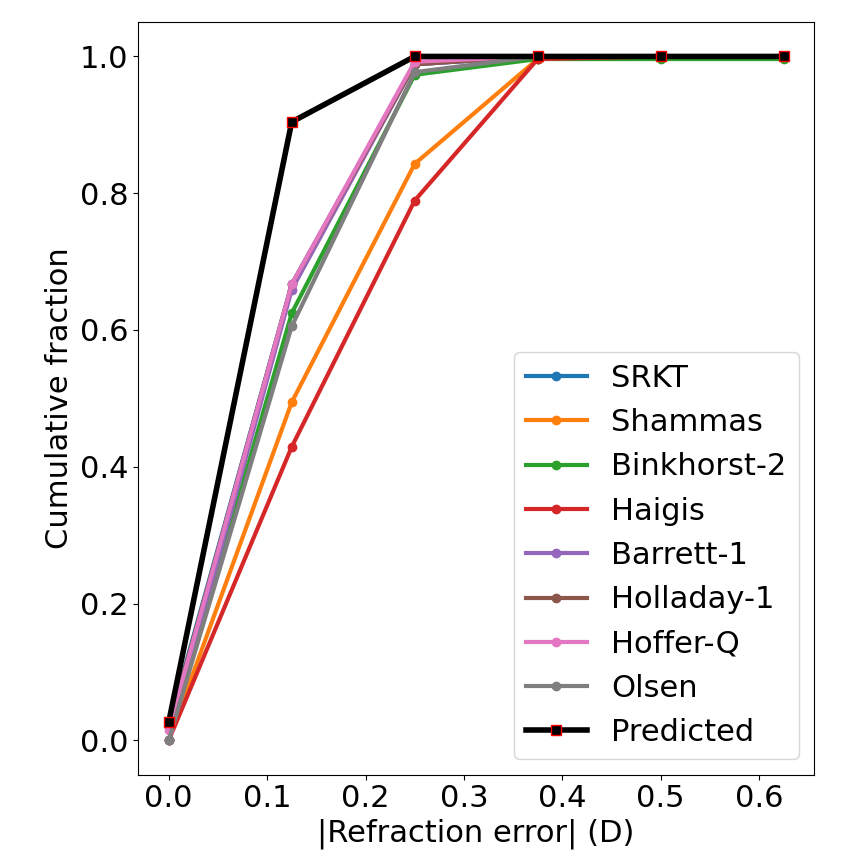
\includegraphics[width=1\linewidth]{cumulativeRefErrAlpha1}
	\caption{Cumulative percentage of observations below an absolute refraction error $|R_f-R|$ in intervals of 0.125D, shows our prediction method (black) is superior to the 8 IOL formulas tested, with 92\% of observations below 0.125D error using our prediction method.}
	\label{fig:cumulativereferralpha1}
\end{figure}


In Figure \ref{fig:RefErrVsAxialLengthAlpha1} we plot the refraction error $|R_f-R|$ as a function of the axial length, showing that our predictions (red circle) are all within the range $\pm0.125D$.
\begin{figure*}
	\centering
	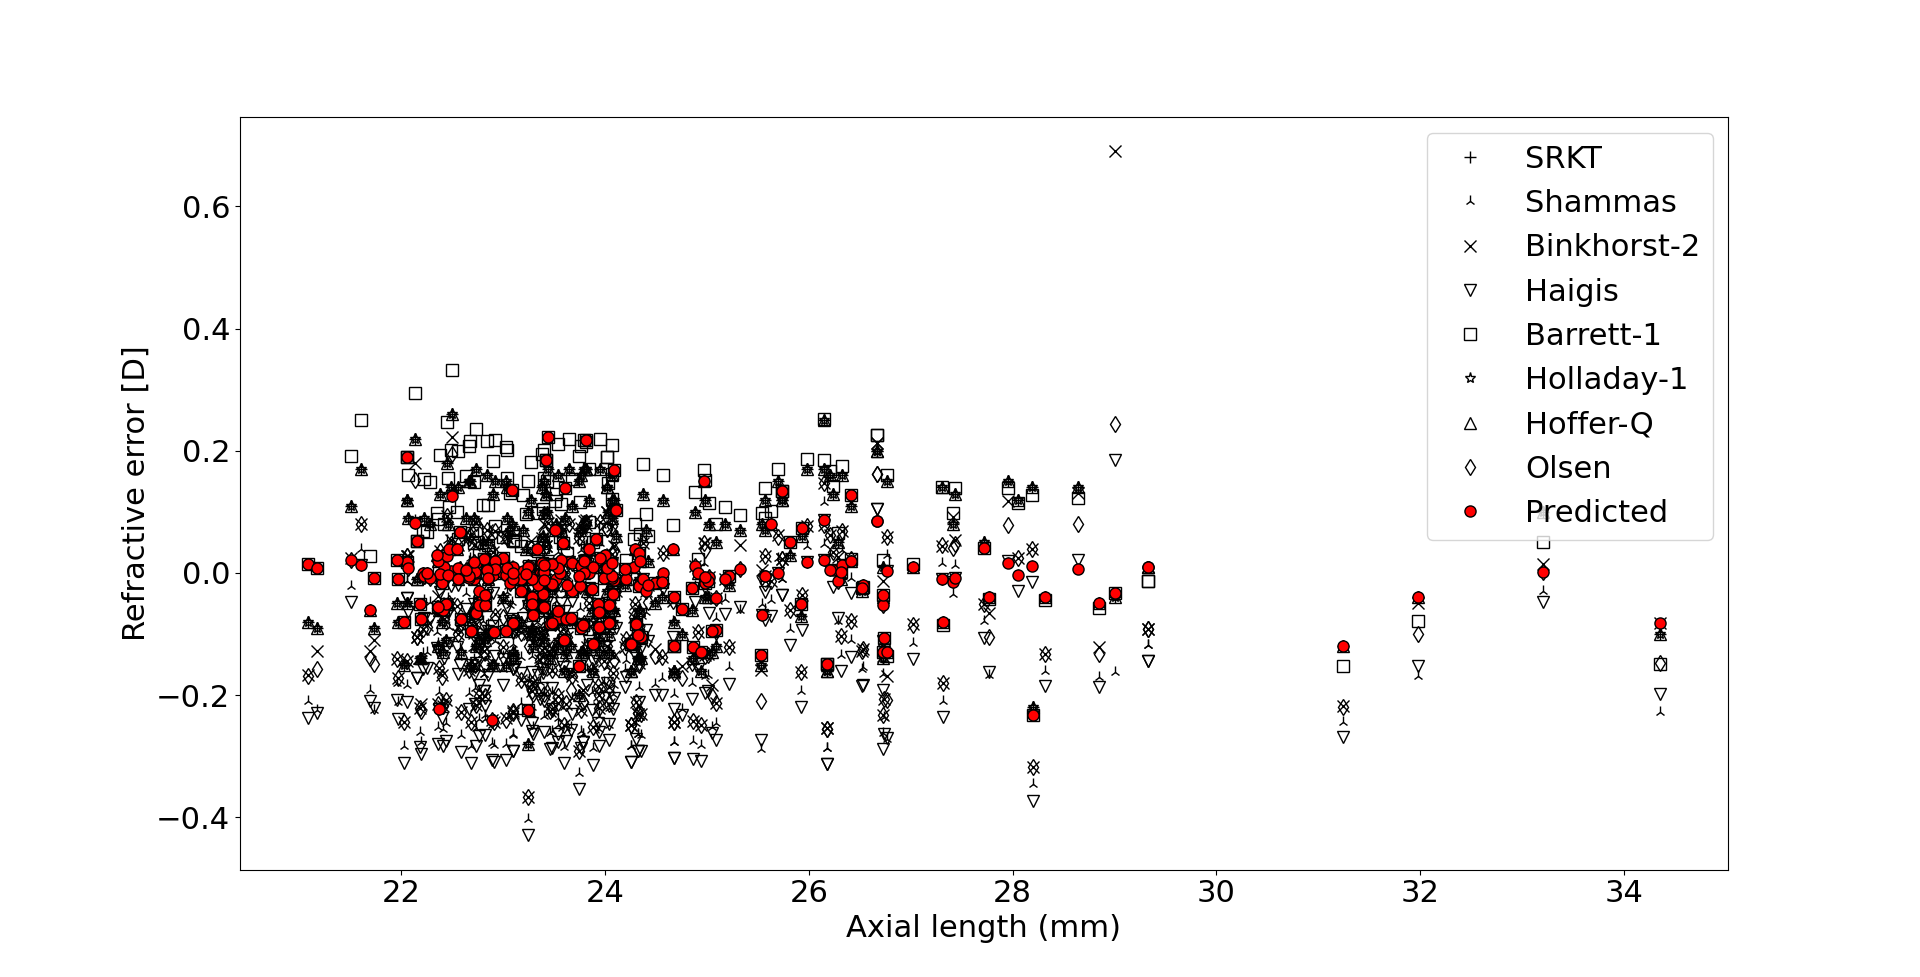
\includegraphics[width=1\linewidth]{RefErrVsAxialLength_alpha1}
	\caption{Refraction error $R_f-R$ as a function of the axial length. Our predictions in red circles, showing a consistent refraction error in the range of $\pm0.125D$ for all values of the axial length.}
	\label{fig:RefErrVsAxialLengthAlpha1}
\end{figure*}

Next, we tested the contribution of the subjective factor in Eq \ref{eq:goalFunctionRefractionPower} for various values $0<\alpha<1$. We tested various value and obtained that a value of $\alpha=0.6$ provides a good balance between the accuracy of the prediction, and minimizes simultaneously both the refraction error and the power error. In Table \ref{} we summarize the cumulative fraction of observations falling below a certain refraction error threshold. 


\begin{figure*}
	\centering
	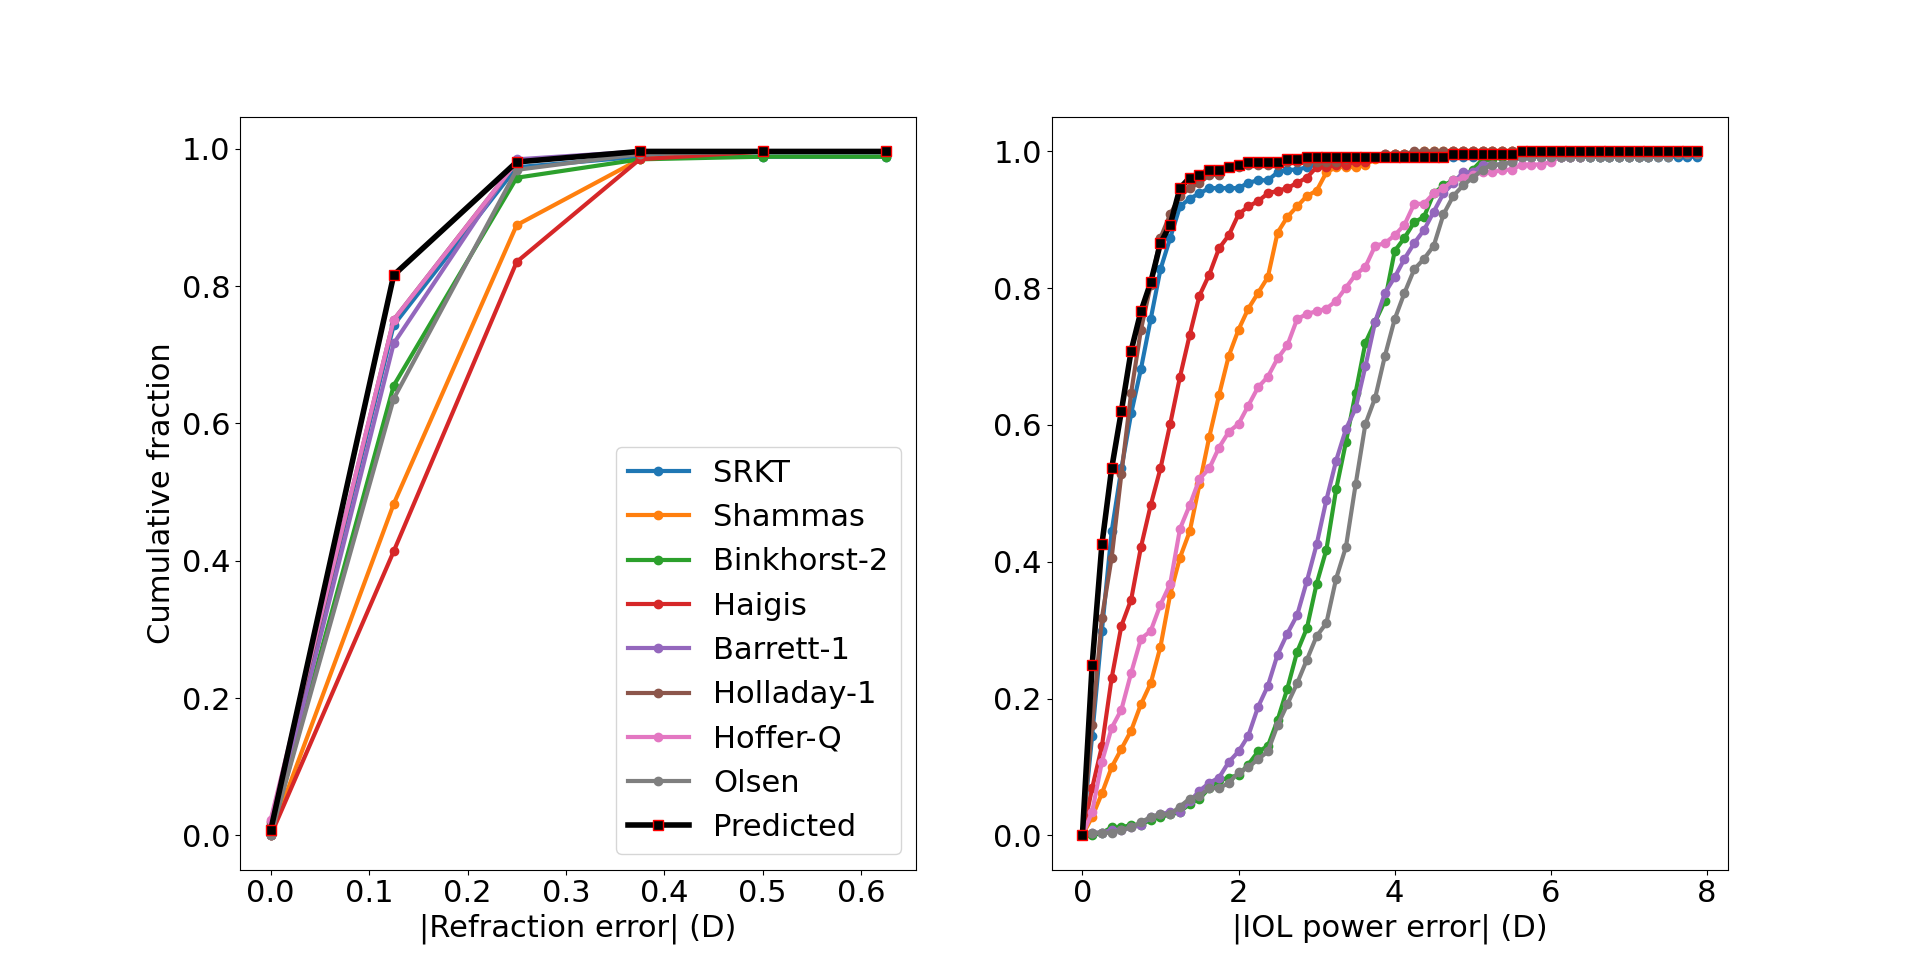
\includegraphics[width=1\linewidth]{powerAndRefErr_alpha0_6}
	\caption{Cumulative fraction of observations below a certain refraction error (left panel) and below certain power error (right panel). Our prediction method appears in black. using our prediction methods for $\alpha=0.6$, 82\% of predictions fall below refraction error of 0.125D and }
	\label{fig:PowerAndRefErrAlpha06}
\end{figure*}

\section{Discussion}\label{section:Discussion}
\red{TODO: finish section}

\section{Appendix}\label{section:iolFormulas}
\subsection{Computational tools}
All codes were written inPython 3.8 using the machine learning package Sklearn. 
All computations were performed by an in-house codes.

\subsection{Parameters of the trained classifier}\label{subsection:parametersOfClassifier}
Parameters used for the RF classifier are summarized in Table \ref{table:parametersOfTheRFclassifier}. We examined a range of the hyper-parameters and found the listed ones a good compromise between size of the forest and the risk of over fitting the training data. The parameter names appears as in the sklearn package in Python.
\begin{table}
	\begin{tabular}{l|c}
		Parameter     & Value \\
		\hline 
		\hline
		n estimators  & 70 \\
		criterion     & entropy \\
		max. depth    & 150 \\
		ccp alpha     & 1e-6\\
		max. features & 3
	\end{tabular}
\label{table:parametersOfTheRFclassifier}
\caption{The random forest classifier parameters used for training. Parameter names appearing here match the nomenclature of the sklearn Python package.}
\end{table}

Below, we summarize the calculation steps required for implementing the 8 formulas used in this research. The steps outlined in the next few subsections might differ in some parts from steps in the original publications of the methods. These modifications were made due to the presence of printing errors appearing in the original publications, corrected here.

\subsection{SRK}\label{subsection:srk}
The SRK IOL power calculation method is performed using the empirical regression formula
\beq
P = Aconst-0.9*\bar{K}-2.5*L,
\eeq 
with $P$ the IOL power (D), Aconst- the IOL manufecturer A-constant, $\bar{K}$ mean keratometry (D), and $L$ the axial length (mm).

To compute the resulting refraction 
\beq
R = P-1.5R_t,
\eeq 
with $R_t$ the target refraction (D)
The A-constant should be adjusted using retrospective data as follows:
\red{TODO: complete estimation of the A-const retrospectively}

\subsection{SRK/T}\label{subsection:srkt}
Set the refractive index $n_c=1.3375$. Start with a retrospective data computation of the individualized (surgeon) A-constant, or the $A_{indiv}$
\begin{enumerate}
	\item Use implanted power $P$, mean keratometry $K = 337.5/R_c$, measured axial length $L$, obtain refraction post op $R$ and compute the refraction factor $\rho$ as
	\beq 
	\rho =\begin{cases} 
		 1.25, & P>16;\\ 
		 1, & P \leq 16
		\end{cases}
	\eeq 
	\item Compute the correction factor $C$ for short and long eyes 
	\beq 
	C = \begin{cases}
		-0.5, & L>24;\\
		0, & 22\leq L\leq24;\\
		1, & 21 \leq L<22;\\
		2, & 20\leq L<21;\\
		3, & L<20.
	\end{cases}
	\eeq 
	\item For each observation, compute the individualized A-constant 
	\beq 
	A_{i} = P_i+\rho R_f+2.5L+0.9K-C,
	\eeq 
	\item Compute the average of $A_i$ over all observations $i$, to obtain the individualized A-constant
	\beq 
	A_{indiv} = \langle A_i\rangle
	\eeq 
\end{enumerate}

Then, use retrospective data to compute  the mean cornea height $H$ by the following steps:
\begin{enumerate} 
	\item Apply correction to the axial length $L$ to obtain $L_c$
	\beq 
	 L_c = \begin{cases}
	 	L, & L\leq 24.4;\\
	 	-3.446 +1.716L-0.0237L^2, & L>24.4.
	 \end{cases}
	\eeq 
	\item For each observation in the retrospective data, compute the cornea width $C_w$ 
	\beq
	 C_w = - 5.41 + 0.58412L_c + 0.098K.
	\eeq 
	\item Compute corneal height,
	\beq 
	   C_h = R_c-\sqrt{R_c^2 -0.25C_w^2}
	\eeq 
	\item compute $H=\langle C_h\rangle$ as the mean corneal height 	
\end{enumerate}

The steps for computing the SRK/T IOL power for each observation are as follows: 
\begin{enumerate} 
\item Adjust the measured axial length $L$ to obtain the corrected $L_c$ in the following manner 
\beq 
L_c = \begin{cases}
	L, & L\leq 24.4;\\
	-3.36+1.716L-0.0237L^2, & L>24.4.
\end{cases}
\eeq 
\item Compute the retina thickness $r_t$ 
\beq 
 r_t = 0.65696-0.02029L
\eeq 
\item compute the optical axial length $L_{opt}$
\beq 
 L_{opt} = L_c+rt;
\eeq 
\item Compute the mean keratometry $K = 0.5(K_1+K_2)$;
\item Compute the mean corneal radius $Rc = 337.5/K$;
\item Compute the corneal width $C_w$ 
\beq 
C_w = -5.41+0.58412L_c+0.098K;
\eeq 
\item Compute corneal height $C_h$
\beq 
 C_h = Rc-\sqrt{Rc^2- 0.25C_w^2};
\eeq 
\item Compute the $ACD_{const}$ from the $A_{const}$
\beq 
 ACD_{const} = 0.62467A_{const}-68.747.
\eeq 
The $ACD_{const}$ can also be computed using the personalized A-constant, $A_{indiv}$ as described above; 
\item Compute the cornea height offset term 
\beq 
offset = ACD_{const}-\langle C_h\rangle. 
\eeq 
A default value for the mean corneal height is 3.336.
\item Compute the ELP $e$
\beq 
e = C_h+offset.
\eeq 
\item Compute the IOL power $P$ at the spectacle plane 
\beq 
 P = \frac{1000n_a(n_aR_c-(n_c-1)L_{opt}-0.001Rx(v(n_aR_c-(n_c-1)L_{opt})+L_{opt}R_c))}{(L_{opt}-e)(n_aR_c-(n_c-1)e-0.001Rx(v(n_aR_c-(n_c-1)e)eR_c))}.
\eeq 
\item Compute the expected refraction $R$
\beq 
R = \frac{1000n_a(n_aR_c-(n_c-1)L_{opt})-P(L_{opt}-e)(n_aR_c-(n_c-1)e)}{n_a(v(n_aR_c-(n_a-1)L_{opt})+L_{opt}R_c)-0.001P(L_{opt}-e)(v(n_aR_c-(n_c-1)e)+eR_c) }.
\eeq 
\item translate refraction to the cornea plane by
\beq 
R \leftarrow \frac{R}{1+vR}
\eeq  

\end{enumerate}


\subsection{Binkhorst}\label{subsection:Binkhorst}
\beq 
P = \frac{1336(4\frac{337.5}{K+R_t}-a)}{(a-e)\left(4\frac{337.5}{k+R_t}-e\right)}
\eeq 
\subsection{Fyodorov}\label{subsection:Fyodorov}s
\beq 
P  = \frac{1336-a(K+R_t)}{(a-e)\left(1-\frac{e(K+R_t)}{1336}\right)}
\eeq 


\subsection{Holladay I}\label{subsection:Hollady1}
\textbf{Input}: $K$, mean keratometry (D), $a$- the axial length (mm), $A_c$ the IOL A constant, $n_c$- index of refraction of the cornea, $n_v$ index of refraction of the vitreous, $R_t$ target refraction (D).
\begin{enumerate}	
	\item Compute $R_c$ the radius of the cornea (mm) by $R_c=337.5/K$:
	\item Set $R_c = \begin{cases}R_c, & Rc\geq 7.7mm;\\
	7.7, & Rc<7.7mm \end{cases}$.
	\item Correct the axial length by \beq a\leftarrow a+0.2 \nonumber \eeq
	\item set \beq a= \begin{cases}a, & a\leq 25.326\\25.326, & a>25.326\end{cases}\eeq
	\item Compute the predicted ACD by:
	\beq aACD=0.56+R_c-\sqrt{R_c^2-a^2/14.077504} \nonumber\eeq 
	\item Set the default value for the surgeon factor \beq s=0.5663*A_c-65.6 \nonumber \eeq
	\item if a computation of the surgeon factor is needed, follow the steps in \ref{subsubsection:theSurgeonFactor};
	\item Compute $e$ the ELP as \beq e=s+aACD \nonumber \eeq.
	\item Compute $P$ the IOL power by:
	\beq P= \frac{n_v}{a-e}-\frac{n_c}{\frac{n_c}{K+R_t}-e} \eeq.
\end{enumerate}

\subsubsection{Computing the Surgeon factor $s$}\label{subsubsection:theSurgeonFactor}
Retrospective computation of the Holladay surgeon factor using post-operative data.\\
\textbf{Input:} $P$- implanted IOL power (D), $R_r$- final refraction (D), $K$- mean keratometry (D), $a$- axial length (mm), set $n_c=n_v=4/3, v=0.012m$. The steps below should be performed for each value of $K$, $a$, $P$, and $R_r$:
\begin{enumerate}
	\item $\forall K$, compute the radius of the cornea \beq R_c = 337.5/K \nonumber \eeq.
	\item $\forall R_c$ set \beq R_c = \begin{cases}R_c, & R_c\geq 7\\
	7,& R_c<7mm\end{cases}\eeq 
	\item Compute the anatomical ACD \beq acd = 0.56+R_c-\sqrt{R_c^2 -a^2/14.077504}\eeq
	\item Correct the axial length by \beq a\leftarrow a+0.2 \eeq
	\item 
	For each value of $R_c$, $acd$, $a$, compute the individualized surgeon factor as by following the steps:
	\beq 
	  q_1 &=& n_v-1 - R_r(v(n_e-1)-R_c)\nonumber \\
	  q_2 &=& R_cv(n_vR_c-an_c) \nonumber \\
	  q_3 &=& R_r(vN_cR_c+a(R_c-v(n_v-1))) \nonumber \\
	  q_4 &=& nc(aR_c(1-vR_r)-(n_cR_c-a(n_v-1)-q_3)/\pi )\nonumber \\
	  s  &=& (-q_2-\sqrt{q_2^2-4q_1q_4})/(2q_1)-acd  
	\eeq 
	\item Compute the average of the individualized surgeon factor $s$, and set it as the new surgeon factor 
\end{enumerate}

\section{Relationship between ACD and axial length}
\red{TODO: finish subsection}

\section{Computing refraction from IOL power prediction}
After the IOL power $P$ is predicted using any formula, the refraction $R_s$ (sphere only) can be computed and used as a measure of error with observed refraction
\beq 
R_s = \frac{1336(4R_c-a)-P(a-d)(4R_c-d)}{1336(v(4R_c-a)-0.003aR_c)-P(a-d)(v(4R_c-d)+0.003dR_c)}
\eeq
\bibliographystyle{plain}
\bibliography{IOLPredictionSummary.bib}

\end{document}

